\let\negmedspace\undefined
\let\negthickspace\undefined
\documentclass[journal]{article}
\usepackage[a5paper, margin=10mm, onecolumn]{geometry}
\usepackage{lmodern} % Ensure lmodern is loaded for pdflatex

\setlength{\headheight}{1cm} % Set the height of the header box
\setlength{\headsep}{0mm}     % Set the distance between the header box and the top of the text

\usepackage{gvv-book}
\usepackage{gvv}
\usepackage{cite}
\usepackage{textcomp}
\usepackage{amsmath,amssymb,amsfonts,amsthm}
\usepackage{algorithmic}
\usepackage{graphicx}
\graphicspath{{./figs/}}
\usepackage{textcomp}
\usepackage{xcolor}
\usepackage{txfonts}
\usepackage{listings}
\usepackage{enumitem}
\usepackage{mathtools}
\usepackage{gensymb}
\usepackage{comment}
\usepackage[breaklinks=true]{hyperref}
\usepackage{tkz-euclide} 
\usepackage{listings}
\usepackage{gvv}                                        
\def\inputGnumericTable{}                                 
\usepackage[latin1]{inputenc}                                
\usepackage{color}                                            
\usepackage{array}                                            
\usepackage{longtable}                                       
\usepackage{calc}                                             
\usepackage{multirow}                                         
\usepackage{hhline}                                           
\usepackage{ifthen}                                           
\usepackage{lscape}
\usepackage{circuitikz}
\tikzstyle{block} = [rectangle, draw, fill=blue!20, 
text width=4em, text centered, rounded corners, minimum height=3em]
\tikzstyle{sum} = [draw, fill=blue!10, circle, minimum size=1cm, node distance=1.5cm]
\tikzstyle{input} = [coordinate]
\tikzstyle{output} = [coordinate]


\begin{document}
	
	\bibliographystyle{IEEEtran}
	\vspace{3cm}
	
\title{4.13.51}
\author{EE25BTECH11047 - RAVULA SHASHANK REDDY}
\maketitle
\hrulefill
\bigskip 

\renewcommand{\thetable}{\theenumi}
\setlength{\intextsep}{10pt}

\textbf{Question:} \\

One of the diameters of the circle circumscribing the rectangle \(ABCD\) is given by
\begin{align*}
4y = x + 7.
\end{align*}

If \(\vec{A}=(-3,4)\) and \(\vec{B}=(5,4)\), find the area of the rectangle.\\

\textbf{Solution:}\\

Circle equation : \quad Centre $\vec{O}=-\vec{u}=-\myvec{u_1\\u_2}$
\begin{align}
\|\vec{x}\|^2 + 2 \vec{u}^\top \vec{x} + f = 0\\
\|\vec{A}\|^2 + 2 \vec{u}^\top \vec{A} + f = 0\\
\|\vec{B}\|^2 + 2 \vec{u}^\top \vec{B} + f = 0
\end{align}

Diameter equation:(Centre lies on diameter)
\begin{align}
\myvec{1 \\ -4}^T\vec{x}=-7\\
\vec{n}^T\vec{u}=c\\
\myvec{2\vec{A} & 2\vec{B} & n \\ 1 & 1 & 0}^T\myvec{\vec{u}\\f}=-\myvec{||\vec{A}||^2\\||\vec{B}||^2\\c}\\
\myvec{-6 & 10 & 1  \\
8 & 8 & -4 \\
1 & 1 & 0 }^T\myvec{\vec{u}\\f} = -\myvec{25 \\ 41 \\ -7}\\
\myvec{
-6 & 8 & 1 & -25 \\
10 & 8 & 1 & -41 \\
1 & -4 & 0 & 7
}
\xrightarrow{ R_1 \leftrightarrow R_3} & \quad
\myvec{
1 & -4 & 0 & 7 \\
10 & 8 & 1 & -41 \\
-6 & 8 & 1 & -25
} 
\end{align}
\begin{align}
R_2 \to R_2 - 10R_1, \; R_3 \to R_3 + 6 R_1 :
 \myvec{
1 & -4 & 0 & 7 \\
0 & 48 & 1 & -111 \\
0 & -16 & 1 & 17
} \\
R_3 \to R_3 + \frac{1}{3} R_2 :
 \myvec{
1 & -4 & 0 & 7 \\
0 & 48 & 1 & -111 \\
0 & 0 & 4/3 & -20
}
\end{align}

\begin{align}
\frac{4}{3} f &= -20 \implies f = -15 \\
48 u_2 + f &= -111 \implies 48 u_2 - 15 = -111 \implies u_2 = -2 \\
u_1 - 4 u_2 &= 7 \implies  u_1 = -1\\
\vec{u} &= \myvec{-1 \\ -2}, \quad f = -15\\
\vec{O} &= -\vec{u} = \myvec{1 \\ 2}
\end{align}
Equation of the Circumcircle:
\begin{align}
\boxed{||\vec{x}||^2+2\myvec{-1 & -2}\vec{x}-15=0}
\end{align}
\begin{align}
\vec{C} &= 2\vec{O} - \vec{A} = 2\myvec{1 \\ 2} - \myvec{-3 \\ 4} = \myvec{5 \\ 0} \\
\vec{D} &= 2\vec{O} - \vec{B} = 2\myvec{1 \\ 2} - \myvec{5 \\ 4} = \myvec{-3 \\ 0}
\end{align}
\begin{align}
\text{Area}=|(\vec{B} - \vec{A}) \times (\vec{D} -\vec{A})| =
\begin{vmatrix} 8 & 0 \\ 0 & -4 \end{vmatrix} = 32
\end{align}

\newpage
\begin{figure}
    \centering
    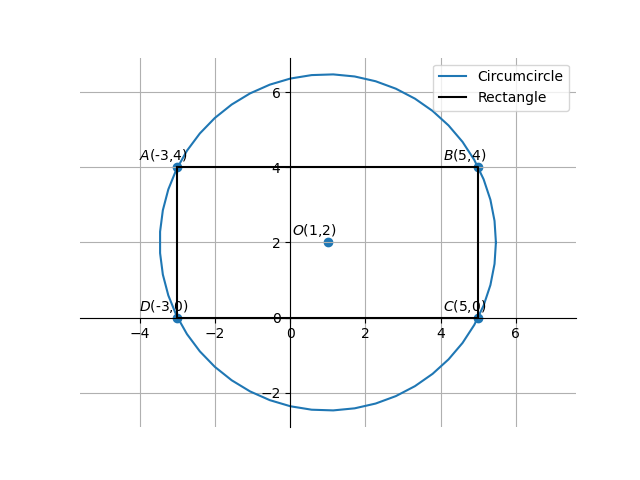
\includegraphics[width=1.0\linewidth]{figs/fig1.png}
    \caption{}
    \label{fig:placeholder}
\end{figure}
\end{document}